% Full-length journal draft. Finite certificate inputs are attributed, not newly replayed.
\documentclass[11pt,a4paper]{article}
\usepackage[margin=25mm,headheight=14pt]{geometry}
\usepackage[T1]{fontenc}
\usepackage{lmodern,microtype,amsmath,amssymb,amsthm,mathtools}
\usepackage{booktabs,array,longtable,enumitem,tikz,fancyhdr}
\usetikzlibrary{arrows.meta,positioning}
\usepackage[colorlinks=true,linkcolor=blue!45!black,citecolor=blue!45!black,urlcolor=blue!45!black,hypertexnames=false]{hyperref}
\setlength{\emergencystretch}{2em}
\setlength{\parskip}{3pt}
\setlist{nosep,leftmargin=1.6em}
\pagestyle{fancy}\fancyhf{}
\fancyhead[L]{\small Three-copy qutrit Werner endpoint}
\fancyhead[R]{\small Research article draft}
\fancyfoot[C]{\thepage}
\newtheorem{theorem}{Theorem}
\newtheorem{proposition}[theorem]{Proposition}
\newtheorem{lemma}[theorem]{Lemma}
\newtheorem{corollary}[theorem]{Corollary}
\theoremstyle{definition}\newtheorem{definition}[theorem]{Definition}
\theoremstyle{remark}\newtheorem{remark}[theorem]{Remark}
\DeclareMathOperator{\Tr}{Tr}\DeclareMathOperator{\rank}{rank}
\DeclareMathOperator{\ran}{ran}\DeclareMathOperator{\vecop}{vec}
\DeclareMathOperator{\Alt}{Alt}\DeclareMathOperator{\diag}{diag}
\DeclareMathOperator{\dist}{dist}
\newcommand{\C}{\mathbb C}\newcommand{\R}{\mathbb R}
\newcommand{\HH}{\mathcal H}\newcommand{\LL}{\mathcal L}
\newcommand{\nf}[1]{\lVert#1\rVert_F}
\newcommand{\hs}[1]{\lVert#1\rVert_{\mathrm{HS}}}
\newcommand{\op}[1]{\lVert#1\rVert_{\mathrm{op}}}
\newcommand{\ip}[2]{\langle#1,#2\rangle}
\newcommand{\ket}[1]{|#1\rangle}\newcommand{\bra}[1]{\langle#1|}
\newcommand{\dd}{\mathrm d}
\numberwithin{equation}{section}
\hypersetup{pdftitle={Three-copy undistillability of qutrit Werner states by an intrinsic positive identity},pdfauthor={Physical Superintelligence},pdfsubject={Full-length research article draft}}
\title{\bfseries Three-copy undistillability of qutrit Werner states\\
by an intrinsic positive identity}
\author{Physical Superintelligence}
\date{17 September 2026}
\begin{document}
\maketitle
\begin{abstract}
We present a finite-certificate proof of three-copy undistillability
for the qutrit Werner state $(2I_9-F)/15$, where $F$ exchanges the
two qutrits. Equivalently, an alternating partial-trace quadratic
form is nonnegative on every complex $27\times27$ matrix of rank
at most two, with no normality or common-support assumption.
The proof is expressed intrinsically through the second compound
$M(C)=\bigwedge^2C$. Three fixed positive Gram operators give a
sum-of-squares identity for $\|M(C)\|_F^4q_{1/2}(C)$.
Physical zeros determine the Gram supports; exact range compatibility,
a rational positive trial and a certified physical singular-value gap
permit an exact positive correction. We isolate these finite inputs
and prove a sharper correction bound, leaving an explicit mixed-sector
reserve greater than $95/127$ of its certified trial threshold.
The endpoint implies the sharp minimum
$(1-2\alpha)(1-\alpha)^2$ on $0\le\alpha\le1/2$ and the exact
three-copy distillability threshold of the physical qutrit Werner
family. For every fixed pair of support planes, we give four
nonnegative squared moduli and a quantitative description of a
possible zero line. The computational premises and their verification
status are separated from the analytic implications.
\end{abstract}

\noindent\textbf{Draft verification status.}
The finite inputs in Proposition~\ref{prop:finite} are taken from the
existing certificate record \cite{certificate}; this article does
not claim a new independent replay. The complete listed local inventory
has been checked for availability and hash agreement. A public immutable
release and an external mathematical replay are not claimed.
The data availability statement records this boundary.

\section{Introduction}
Entanglement distillation asks whether noisy bipartite entanglement can
be converted, by local operations and classical communication, into
an entangled two-qubit state. Positivity of the partial transpose
precludes distillation. The converse remains a central structural
question: can a state with negative partial transpose remain
undistillable at every finite copy number?
Werner states provide a canonical symmetric setting for this question
\cite{werner,hhh98,dss00}. A finite-copy result has an exact operational
meaning, while retaining a distinction from all-copy undistillability.

The Schmidt-rank-two criterion converts the physical problem into a
matrix inequality. Costa Rico developed the arbitrary-copy partial-trace
formulation \cite{costa}. Recent two-copy results establish coincidence
of the one-copy and two-copy thresholds \cite{fu,song,fraser,bharti}.
The rank-$r$ partial-trace theorem of Fraser, Huber, Pozsgay and Vona
\cite{fraser} supplies the inequality used for our sharp interval
continuation. At three copies, Wu and Zou prove endpoint positivity
for normal rank-two matrices in arbitrary local dimensions, together
with specified nonnormal sectors determined by local support overlap
or a product ray in a support plane \cite{wuzou}.
The contribution considered here is the full complex rank-two domain
when all three local coefficient spaces have dimension three.
The two supporting planes are independent, and the matrices need
not be normal or Hermitian.

The obstruction to a direct quadratic proof is geometric.
The energy form is indefinite on the ambient matrix space, but the
allowed rank-two matrices form a nonlinear variety. The second compound
matrix records the two-dimensional row and column geometry simultaneously.
If $C=XY^*$ with two-column factors, then
\[
\bigwedge\nolimits^2C=(x_0\wedge x_1)(y_0\wedge y_1)^*.
\]
This identity permits an exact transport of a positive polynomial Gram
construction into features depending only on $C$ and its actual minors
\cite{compound}. The transport retains complete complex quadratic
forms, rather than bounding their cross terms separately.

The positive operators arise from a finite construction.
Known physical zeros prescribe exact kernels. Derivatives of these
same zeros produce coefficient relations, which establish compatibility
of the target with a supported transfer map. A rational trial is then
corrected on its prescribed faces. Symmetry reduction and rational
sum-of-squares recovery have established precedents
\cite{gatermann,peyrl}; the task-specific content is the physical
carrier, its forced kernels, the compatible range and the norm control
of the complete correction.

We organize the argument around an explicit distinction.
The analytic theorems show exactly how specified finite predicates
imply the endpoint and its consequences. Proposition~\ref{prop:finite}
states the computational inputs from the existing proof record, and
Appendix~\ref{app:verification} describes their mathematical acceptance
predicates. Hash agreement identifies those data; it does not verify
their mathematical content.

The paired two-qubit construction comes after global positivity.
For any two actual support planes, the compressed swap operator is
strictly positive, and the endpoint makes its logical partial transpose
positive. Two-qubit separability and product-length theorems
\cite{peres,hhh96,sanpera,wootters} then apply. We give bounded filters,
explicit product factors once a normal form is chosen, and a spectral
argument showing that each pair has at most one zero amplitude up to
complex scaling. These local four-term formulas depend on the support
planes; they do not replace the universal polynomial certificate.

\section{Conventions and main statements}\label{sec:statements}
Let $\HH=(\C^3)^{\otimes3}$, with fixed computational product bases.
The tensor factors label resource copies, not three communicating
parties. The physical bipartition is
$A_1A_2A_3:B_1B_2B_3$.
All inner products are conjugate-linear in the first argument, and
all partial traces are unnormalized. Define
\begin{equation}
q_\alpha(C)=\sum_{J\subseteq\{1,2,3\}}(-\alpha)^{|J|}
                   \nf{\Tr_JC}^2,\qquad q=q_{1/2}.
\label{eq:qalpha}
\end{equation}
Here $\Tr_\varnothing C=C$. Thus, writing
$N=\nf C^2$, $A_1=\sum_i\nf{\Tr_iC}^2$,
$B_2=\sum_{i<j}\nf{\Tr_{ij}C}^2$ and $T=|\Tr C|^2$,
\begin{equation}
q(C)=N-\frac12A_1+\frac14B_2-\frac18T.
\label{eq:q}
\end{equation}

\begin{theorem}[Three-copy qutrit endpoint]\label{thm:endpoint}
For every $C\in\operatorname{End}(\HH)$ with $\rank C\le2$,
\begin{equation}
q(C)\ge0.
\label{eq:endpoint}
\end{equation}
The proof uses the finite certificate inputs of
Proposition~\ref{prop:finite}, in their original physical metrics.
\end{theorem}

\begin{corollary}[Sharp interval and physical threshold]\label{cor:interval}
For $0\le\alpha\le1/2$,
\begin{equation}
\min_{\rank C\le2,\ \nf C=1}q_\alpha(C)
=(1-2\alpha)(1-\alpha)^2.
\label{eq:minimum}
\end{equation}
An attainer is
$C_\star=\diag(1,1,0)/\sqrt2\otimes\ket0\bra0\otimes\ket0\bra0$.
For the physical qutrit Werner family
\begin{equation}
\rho_\alpha=\frac{I_9-\alpha F}{9-3\alpha},\qquad -1\le\alpha\le1,
\label{eq:werner}
\end{equation}
three-copy distillability holds exactly when $\alpha>1/2$.
The NPT yet three-copy-undistillable interval is $1/3<\alpha\le1/2$.
\end{corollary}

To verify the physical equivalence, use row-first vectorization,
\[
\vecop C=\sum_{a,b}C_{ab}\ket a_A\ket b_B.
\]
An SVD gives $\vecop C=\sum_j s_ju_j\otimes\overline{v_j}$, so
the Schmidt rank equals $\rank C$. With
$\ket{I_3}=\sum_{j=0}^2\ket{jj}$ and
$\Omega=\ket{I_3}\bra{I_3}$, one has $F^\Gamma=\Omega$.
Contraction with $\bra{I_3}$ at site $i$ gives $\Tr_iC$, hence
\begin{equation}
\ip{\vecop C}{(\rho_\alpha^\Gamma)^{\otimes3}\vecop C}
=\frac{q_\alpha(C)}{(9-3\alpha)^3}.
\label{eq:physical}
\end{equation}
The denominator is positive throughout the physical interval.
The eigenvalue of $\rho_\alpha^\Gamma$ on $\ket{I_3}/\sqrt3$ is
$(1-3\alpha)/(9-3\alpha)$, equal to $-1/15$ at the half endpoint.
These conventions differ in the sign of $\alpha$ from the
$I+\alpha F$ convention used in several cited works.

The rank restriction is essential:
$I_3/\sqrt3\otimes\ket0\bra0\otimes\ket0\bra0$ has rank three,
norm one and energy $-1/8$.

\section{An intrinsic compound identity}\label{sec:intrinsic}
Equip $\bigwedge^2\HH$ with the orthonormal basis
$e_i\wedge e_j=(e_i\otimes e_j-e_j\otimes e_i)/\sqrt2$, $i<j$.
For
\begin{equation}
M(C)=\bigwedge\nolimits^2C,\qquad
M_{(ij),(kl)}=C_{ik}C_{jl}-C_{il}C_{jk},\qquad
\Delta(C)=\nf{M(C)}^2,
\label{eq:compound}
\end{equation}
the singular values of $M(C)$ are $s_is_j$, $i<j$. Therefore
\begin{equation}
\Delta(C)=\frac{(\Tr C^*C)^2-\Tr((C^*C)^2)}2.
\label{eq:delta}
\end{equation}
At rank two, $\Delta=s_1^2s_2^2>0$; at rank at most one, $\Delta=0$.

Let $\mathcal E=\HH\otimes\bigwedge^2\HH\otimes
\bigwedge^2\HH\otimes\HH$ and define
$Z(C;a,b)_{u,I,K,v}=C_{uv}a_Ib_K$.
The second and third factors are exterior coordinates; the matrix
column is in the final slot.

\begin{theorem}[Intrinsic positive identity]\label{thm:intrinsic}
The finite certificate supplies fixed $G_h,G_m,G_a\succeq0$ on
$\mathcal E$, extended by zero from the carriers defined below.
For every $\rank C\le2$, define
\begin{align}
f_{h,JK}&=Z(C;M_J,M_K),&
f_{m,JK}&=Z(C;M_J,\overline{M_K}),&
f_{a,JK}&=Z(C;\overline{M_J},\overline{M_K}).
\label{eq:f}
\end{align}
Here $J,K$ run over the 351 exterior coordinates.
Then
\begin{equation}
\Delta(C)^2q(C)=\sum_{s\in\{h,m,a\}}\sum_{J,K}
                 f_{s,JK}^*G_sf_{s,JK}.
\label{eq:intrinsic}
\end{equation}
Factoring $G_s=R_s^*R_s$ expresses the right side as squared
moduli of polynomials of total degree five.
\end{theorem}

\begin{proof}
At rank two write $C=XY^*$ with two full-column-rank factors.
Set $p=x_0\wedge x_1$, $r=y_0\wedge y_1$ and
$g_X=\|p\|^2$, $g_Y=\|r\|^2$.
Cauchy--Binet gives
\begin{equation}
M=pr^*,\qquad M_J=p\,\overline{r_J},\qquad
\Delta=g_Xg_Y.
\label{eq:cb}
\end{equation}
Both shore incidences hold:
$p\wedge C_{\cdot j}=0$ and $\overline r\wedge C_{i\cdot}=0$,
with the row regarded as a coordinate vector.

The Gram construction of Sections~\ref{sec:gram}--\ref{sec:repair} gives
\begin{align}
z_h&=Z(C;p,p),&z_m&=Z(C;p,\overline p),&
z_a&=Z(C;\overline p,\overline p),\notag\\
g_X^2q(C)&=\sum_s z_s^*G_sz_s.
\label{eq:source}
\end{align}
The complete feature identities are
\[
f_{h,JK}=\overline{r_J}\,\overline{r_K}z_h,\quad
f_{m,JK}=\overline{r_J}r_Kz_m,\quad
f_{a,JK}=r_Jr_Kz_a.
\]
Each quadratic form, including all its internal cross terms, is
multiplied by $|r_J|^2|r_K|^2$. Consequently
\[
\sum_{s,J,K}f_{s,JK}^*G_sf_{s,JK}
=\left(\sum_J|r_J|^2\right)^2\sum_s z_s^*G_sz_s
=g_Y^2g_X^2q(C)=\Delta^2q(C).
\]
At rank at most one both sides vanish. The bidegrees of the three
features in $(C,\overline C)$ are $(5,0),(3,2),(1,4)$.
\end{proof}

This transport is independent of a source frame.
Under $X\mapsto XS$, $Y\mapsto YS^{-*}$,
$p\mapsto(\det S)p$ and
$r\mapsto(\overline{\det S})^{-1}r$, so $M$ and $\Delta$ are unchanged.
The three source features acquire factors
$(\det S)^2$, $|\det S|^2$ and $\overline{\det S}^{\,2}$,
respectively. Every source evaluation scales by $|\det S|^4$,
exactly as $g_X^2q$.

For rank two, \eqref{eq:intrinsic} implies the endpoint by division
by $\Delta^2>0$. At rank one, $C=uv^*$ satisfies the direct identity
\begin{equation}
q(uv^*)=\ip{u\otimes v}{\prod_{i=1}^3(I-F_i/2)\,u\otimes v}
\ge\frac18\|u\|^2\|v\|^2.
\label{eq:rankone}
\end{equation}
The three swaps commute and have eigenvalues $\pm1$.
This proves the rank-one case without division by a vanishing
determinant. An alternative is to extend $\ran C$ to an orthonormal
two-plane in \eqref{eq:source}, making $g_X=1$.

The intrinsic identity inherits the certified Gram operators.
It does not constitute an independent proof of their positivity.

\section{The finite Gram construction}\label{sec:gram}
We use six global $\HH$ slots ordered
$(C\text{ row},p_1,p_2,p'_1,p'_2,C\text{ column})=(0,1,2,3,4,5)$.
Put $A_{ij}=(I-F_{ij})/2$, and let $\Alt_{ijk}$ be the orthogonal
three-slot antisymmetrizer. If $E_\lambda$ denotes the central
Young projector, define
\begin{equation}
\Pi_h=E_{(3,2)}^{(01234)}A_{12}A_{34},\qquad
\Pi_m=(A_{12}-\Alt_{012})A_{34},\qquad
\Pi_a=E_{(2,2)}^{(1234)}A_{12}A_{34}.
\label{eq:carriers}
\end{equation}

\begin{lemma}[Carrier and transpose identities]\label{lem:carriers}
The source features satisfy $\Pi_sz_s=z_s$.
Let $\Gamma_m$ transpose the entire second minor subsystem $3,4$,
and let $\Gamma_a$ transpose the entire subsystem $1,2,3,4$.
For every operator $G$ on the corresponding full tensor space,
\begin{equation}
z_s^*Gz_s=z_h^*\Gamma_s(G)z_h,\qquad s=m,a.
\label{eq:transpose}
\end{equation}
\end{lemma}
\begin{proof}
The pair antisymmetries are immediate. The decomposable tensor
$p\otimes p$ belongs to the Schur module $S_{(2,2)}\HH$.
For a column $c\in\operatorname{span}\{x_0,x_1\}$,
$c\otimes p\otimes p$ lies in $S_{(3,2)}\HH$; equivalently, the
incidence $p\wedge c=0$ removes the three-row component.
The mixed feature satisfies $\Alt_{012}(c\otimes p)=0$.
Appendix~\ref{app:carrierproof} gives direct highest-weight and
finite-projector verifications of these inclusions.

For a fixed split $a\otimes b$, expand
\[
(a\otimes\overline b)^*G(a\otimes\overline b)
=\sum_{i,j,k,l}\overline{a_i}b_jG_{ij,kl}a_k\overline{b_l}.
\]
Interchanging $j,l$ gives the expectation of $\Gamma_b(G)$ on
$a\otimes b$. Apply this to the indicated minor factors.
The matrix coordinate $C_{uv}$ is unchanged.
\end{proof}

Define
\begin{equation}
T_0=\prod_{i=1}^3(I-\Omega_{0_i5_i}/2),\quad
\overline T=\Pi_hT_0\Pi_h,\quad
\mathcal A_s^*(G)=\Pi_h\Gamma_s(G)\Pi_h.
\label{eq:maps}
\end{equation}
The full target identity is
\begin{equation}
\overline T=G_h+\mathcal A_m^*(G_m)+\mathcal A_a^*(G_a),
\qquad G_s\succeq0.
\label{eq:target}
\end{equation}
Transpose precedes compression. It preserves the Hilbert--Schmidt
norm, not positivity. Evaluation on $z_h$, using
$z_h^*T_0z_h=g_X^2q(C)$, gives \eqref{eq:source} with all eight
subset terms and every complex phase retained.

\subsection{Symmetry and the physical metric}
Local-unitary conjugation of $C$, simultaneous site permutations
and complex conjugation preserve the target. Averaging a feasible
Gram tuple over these symmetries preserves positivity and the full
identity. The construction uses a real invariant block ansatz; it
need only exhibit one sufficient certificate.
The local actions in sectors $h,m,a$ have unbarred slot sets
$01234$, $012$, $0$, respectively, with conjugate action on the
remaining slots. These actions are intertwined by the whole-minor
transpose maps.

In a physical isotypic decomposition, a block $G_b$ of multiplicity
$\nu_b$ contributes $\nu_b\Tr(G_b^2)$ to the HS norm.
If $V_b$ is a nonorthonormal native frame, its Gram matrix
$H_b=V_b^*V_b$ must be retained. For $G_b=V_bZV_b^*$,
\[
\Tr(G_b^2)=\Tr(ZH_bZH_b).
\]
No Euclidean coefficient norm replaces this physical quantity.

\subsection{Zeros, faces and exact range}
For any directly verified zero $C_0$, positivity of
\eqref{eq:source} forces $G_sz_s(C_0)=0$ in every sector.
A covariance of zero features therefore defines a necessary support
$P_s\le\Pi_s$ for every feasible $G_s$:
\[
G_s=P_sG_sP_s.
\]
The construction intersects the kernels from product-spectator,
binary spin and qutrit-spectator zero families. Their exact
definitions and nine selected factorizations are in
Appendix~\ref{app:zeros}. The original 414 symmetry blocks leave
327 nonempty faces. Restriction to these faces is necessary; it
does not by itself prove feasibility.

At a selected zero, vary both factors of $C=XB$ through arbitrary
complex directions. With
$J_h=\dot z_hz_h^*+z_h\dot z_h^*$ and $\Gamma_h=\operatorname{Id}$,
\begin{equation}
P_s\Gamma_s(J_h)P_s=0.
\label{eq:relations}
\end{equation}
Both real and imaginary variations are included. Direct full-qutrit
checks of $X^*\LL(C_0)=0$ and $\LL(C_0)B^*=0$ give
$\Tr(J_h\overline T)=\dd(g_X^2q)(C_0)=0$, where
$\LL=(D\mapsto D-\Tr(D)I_3/2)^{\otimes3}$.
Thus the relations annihilate the target without assuming universal
endpoint positivity.

After eliminating the supported $h$ coefficients, let
$\mathsf A$ be the rational transfer with 2463 rows and $t$ its target.
The finite range predicates are
\begin{equation}
L\mathsf A=0,\quad Lt=0,\quad \rank L=181,\quad
\rank\mathsf A\ge2282.
\label{eq:rangepredicates}
\end{equation}
They imply $\ran\mathsf A=\ker L$ and $\rank\mathsf A=2282$.
Nonzero designated minors modulo 65521 certify independence after
checking denominator invertibility. The rational equations, not
modular rank alone, prove target compatibility.
The correction domain retains the designated independent columns.

\section{Positive repair and the finite certificate}\label{sec:repair}
The quantitative refinements below follow the publication review
\cite{review}; their derivations are included. All operator spaces in this
section are real Hilbert spaces of
self-adjoint operators with their physical HS inner products.
Let $\mathcal F_h(H)=P_hHP_h$, $\mathcal Q_h=I-\mathcal F_h$ and
\[
\mathcal C(u_m,u_a)=\mathcal A_m^*(u_m)+\mathcal A_a^*(u_a),\qquad
\mathcal D=\mathcal Q_h\mathcal C|_{\mathcal U}.
\]
The correction domain $\mathcal U$ is supported on the $m,a$ faces.

\begin{lemma}[Orthogonal positive repair]\label{lem:repair}
Let $F$ be an orthogonal projection, $Q=I-F$, $D=Q\mathcal C$
and $\|\mathcal C\|\le\kappa$. Suppose
$QE\in\ran D$, $\|E\|<\varepsilon$ and
$0<\sigma<\sigma_{\min}^+(D)$.
Then
\begin{equation}
u=D^\dagger QE,\qquad v=E-\mathcal Cu
\quad\hbox{satisfy}\quad
Qv=0,\quad
\|u\|<\frac{\varepsilon}{\sigma},\quad
\|v\|<\frac{\kappa\varepsilon}{\sigma}.
\label{eq:repairbounds}
\end{equation}
\end{lemma}
\begin{proof}
Compatibility gives $Du=QE$. Set $x=\|QE\|$, $y=\|FE\|$.
The supported inverse gives $\|u\|\le x/\sigma$. Orthogonality yields
\[
\|F\mathcal Cu\|^2
=\|\mathcal Cu\|^2-\|Q\mathcal Cu\|^2
\le(\kappa^2/\sigma^2-1)x^2.
\]
Since $v=F(E-\mathcal Cu)$, Cauchy--Schwarz gives
\[
\|v\|\le y+\sqrt{\kappa^2/\sigma^2-1}\,x
\le\frac{\kappa}{\sigma}\sqrt{x^2+y^2}
<\frac{\kappa\varepsilon}{\sigma}.
\]
The bracket is nonnegative because
$\sigma<\sigma_{\min}^+(D)\le\|D\|\le\kappa$.
\end{proof}

Let the supported positive trial be $G_s^0$ and retain its complete defect
\begin{equation}
E=\overline T-G_h^0-\mathcal A_m^*(G_m^0)-\mathcal A_a^*(G_a^0).
\label{eq:defect}
\end{equation}

\begin{proposition}[Finite certificate inputs]\label{prop:finite}
The existing certificate record \cite{certificate} supplies the following
finite assertions for the operators and physical coordinates just defined:
\begin{enumerate}[label=(\roman*)]
\item The face projectors and coordinate dictionaries give the stated
414 blocks, 327 nonempty faces and complete full-transpose maps.
\item The exact range predicates \eqref{eq:rangepredicates} hold.
The $11149$-dimensional domain $\mathcal U$ contains the original
2282 independent columns, and $\mathcal Q_hE\in\ran\mathcal D$.
\item Every nonempty trial face has weighted margin greater than
$2^{-13}$, $2^{-18}$, $2^{-15}$ in sectors $h,m,a$, respectively,
and $\|E\|_{\rm HS}<2^{-35}$ on the complete 122-block target.
\item A specified dyadic matrix $A_{48}$ satisfies
$\|\mathcal D-A_{48}\|_{\rm op}<2^{-32}$ in physical orthonormal
coordinates. All 664 transfer blocks are included.
\item The symmetric entrywise grid-rounding $S_{48}$ of
$A_{48}A_{48}^*$ satisfies
$\|A_{48}A_{48}^*-S_{48}\|_{\rm op}<2463\,2^{-48}$ and
$\lambda_{182}(S_{48})>2^{-30}$, with eigenvalues increasing.
\end{enumerate}
These are attributed computational inputs, not conclusions of the
small diagnostic examples below. Their acceptance predicates and
present verification status are specified in
Appendix~\ref{app:verification}.
\end{proposition}

\begin{lemma}[Sharpened physical gap]\label{lem:gap}
The finite inputs imply
\begin{equation}
\sigma_{\min}^+(\mathcal D)>
\sqrt{259681}\,2^{-24}-2^{-32}>127\,2^{-22}.
\label{eq:gap}
\end{equation}
\end{lemma}
\begin{proof}
Eigenvalue perturbation gives
$s_{182}(A_{48})^2>2^{-30}-2463\,2^{-48}=259681\,2^{-48}$.
Singular-value perturbation subtracts at most $2^{-32}$.
Exact rank $2282$ in 2463 output dimensions makes the 182nd
singular value the least positive one. The last comparison follows
by squaring positive quantities:
\[
259681-(508+1/256)^2=105711615/65536>0.
\]
\end{proof}

Full transpose is an HS isometry and compression a contraction,
so $\|\mathcal C\|\le\sqrt2$.
Apply Lemma~\ref{lem:repair} with
$\varepsilon=2^{-35}$ and $\sigma=127\,2^{-22}$:
\begin{align}
u&=\mathcal D^\dagger\mathcal Q_hE,\notag\\
G_m&=G_m^0+u_m,\quad G_a=G_a^0+u_a,\quad
G_h=G_h^0+E-\mathcal Cu.
\label{eq:exactrepair}
\end{align}
The supports are preserved because
$\mathcal Q_h(E-\mathcal Cu)=0$, and \eqref{eq:target} holds by
substitution. With $b=2^{-18}$, the corrections obey
$\|u\|<(32/127)b$ and
$\|G_h-G_h^0\|<(32\sqrt2/127)b<(48/127)b$.
Since $\sqrt{\nu_b}\|\delta G_b\|_{\rm op}\le\|\delta G_s\|_{\rm HS}$,
every face remains positive with the explicit margins in
Table~\ref{tab:margins}.

\begin{table}[ht]
\centering
\begin{tabular}{@{}lccc@{}}
\toprule
Sector & Trial weighted margin & Correction bound & Corrected margin\\
\midrule
$h$ & $>32b$ & $<(48/127)b$ & $>(4016/127)b$\\
$m$ & $>b$ & $<(32/127)b$ & $>(95/127)b$\\
$a$ & $>8b$ & $<(32/127)b$ & $>(984/127)b$\\
\bottomrule
\end{tabular}
\caption{All nonempty faces, with $b=2^{-18}$ and original physical
multiplicities. Empty faces remain empty. The improved bounds use
the existing finite inputs without another large computation.}
\label{tab:margins}
\end{table}

The exact correction has a rational native specification.
If $E_j$ are native source atoms,
$M_{\mathcal U,ij}=\Tr(E_iE_j)$, and $D_I,e_I$ restrict the transfer
and defect to the independent rows, then
\begin{equation}
c=M_{\mathcal U}^{-1}D_I^T
 (D_IM_{\mathcal U}^{-1}D_I^T)^{-1}e_I,\qquad u=\sum_jc_jE_j.
\label{eq:rational}
\end{equation}
Both inverses are ordinary positive inverses.
Lagrange multipliers identify this as the unique minimum of
$c^TM_{\mathcal U}c$ subject to $D_Ic=e_I$.
Exact compatibility supplies every remaining row. An invertible
change of output coordinates leaves this constrained minimum unchanged;
the source metric, including its cross entries, cannot be omitted.

Equations~\eqref{eq:exactrepair} and \eqref{eq:rational} therefore
specify an exact positive tuple. Lemma~\ref{lem:carriers} gives
\eqref{eq:source}; Theorem~\ref{thm:intrinsic} and
\eqref{eq:rankone} complete Theorem~\ref{thm:endpoint}.

\begin{figure}[ht]
\centering
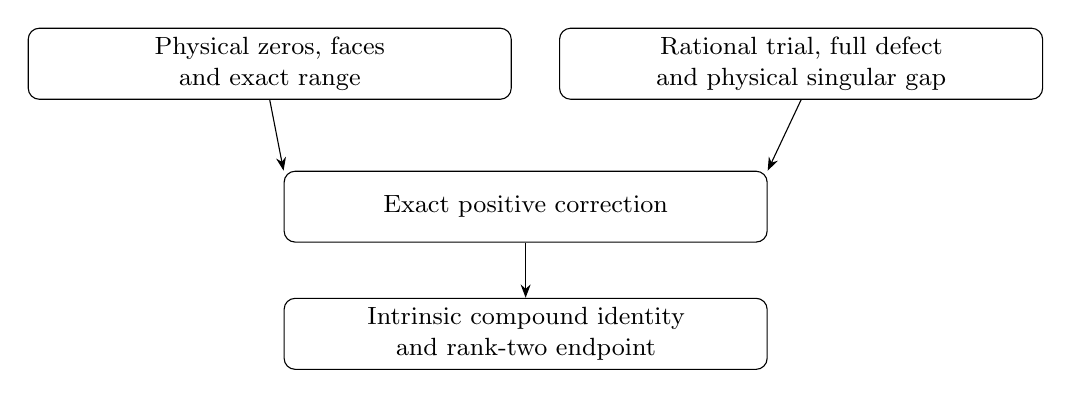
\begin{tikzpicture}[font=\small,>=Stealth,
box/.style={draw,rounded corners,align=center,minimum height=9mm,text width=5.9cm}]
\node[box] (r) {Physical zeros, faces\\and exact range};
\node[box,right=6mm of r] (n) {Rational trial, full defect\\and physical singular gap};
\node[box,below=9mm of r,xshift=3.25cm] (p) {Exact positive correction};
\node[box,below=7mm of p] (i) {Intrinsic compound identity\\and rank-two endpoint};
\draw[->] (r.south)--(p.north west);
\draw[->] (n.south)--(p.north east);
\draw[->] (p)--(i);
\end{tikzpicture}
\caption{The range and quantitative branches meet on the same
physical operators. The paired four-square representation is a
consequence of the endpoint, not an input to this diagram.}
\end{figure}

\section{Sharp continuation and the Werner threshold}\label{sec:interval}
For the same rank-two matrix throughout, set
\begin{equation}
R_3=N-\frac T2,\qquad
R_{12}=N-\frac{A_1+B_2}{6}+\frac T4.
\label{eq:reserves}
\end{equation}
The nuclear trace bound gives $R_3\ge0$.
The rank-two instance of the partial-trace inequality of
Fraser et al.~\cite{fraser} is
\begin{equation}
\|\Tr_LC\|_F^2+\|\Tr_RC\|_F^2
\le2\|C\|_F^2+\frac12|\Tr C|^2.
\label{eq:two}
\end{equation}
Apply it on each of the three actual $3$-by-$9$ regroupings of $C$
and sum, obtaining $R_{12}\ge0$. Regrouping preserves global rank;
a partial trace need not preserve it. A direct proof of the needed
rank-two inequality is included in Appendix~\ref{app:two}.

Coefficient comparison gives the exact identity
\begin{align}
q_\alpha(C)={}&(1-2\alpha)(1-\alpha)^2N
+\frac{4\alpha(1+\alpha)}3q(C)\notag\\
&+\alpha(1-2\alpha)(2/3-\alpha)R_3
+2\alpha(1-2\alpha)R_{12}.
\label{eq:continuation}
\end{align}
All coefficients are nonnegative on $[0,1/2]$.
The matrix $C_\star$ in Corollary~\ref{cor:interval} has invariants
$(N,A_1,B_2,T)=(1,4,5,2)$ and attains the claimed minimum.

For $\alpha\le0$, each factor $I-\alpha\Omega$ is positive.
For $\alpha>1/2$, the rank-two unit matrix
\begin{equation}
C_>=\frac{\diag(1,1,0)}{\sqrt2}
       \otimes\ket0\bra1\otimes\ket0\bra1
\label{eq:above}
\end{equation}
has invariants $(1,2,0,0)$ and energy $q_\alpha(C_>)=1-2\alpha<0$.
This remains negative at $\alpha=1$.
Together with \eqref{eq:physical}, these observations prove the full
physical threshold. Padding a lower-copy witness by
$\ket0\bra0$ multiplies its energy by $1-\alpha$ and preserves rank,
so endpoint nonnegativity also includes the one-copy and two-copy tests.

\section{Consequences on fixed support planes}\label{sec:pair}
Let $U,V:\C^2\to\HH$ be arbitrary isometries.
For $C=UAV^*$, $A\in M_2(\C)$, define
\begin{equation}
D=(U\otimes V)^*\prod_{i=1}^3(I-F_i/2)(U\otimes V),
\qquad K=D^\Gamma.
\label{eq:paired}
\end{equation}
The swaps act between the two global replicas, and $\Gamma$
transposes the second logical qubit.
One always has $D\succeq I_4/8$.
In logical coordinates, $K_{ab,cd}=D_{ad,cb}$.
Contracting with $\overline{A_{ab}}A_{cd}$ gives
\begin{equation}
q(UAV^*)=(\vecop A)^*K\vecop A.
\label{eq:pairenergy}
\end{equation}
Theorem~\ref{thm:endpoint}, applied to every amplitude $A$, therefore
gives $K\succeq0$.

\subsection{An unconditional spectral gap and zero geometry}
\begin{proposition}[Fixed-plane geometry]\label{prop:geometry}
With eigenvalues increasing, $\lambda_2(K)\ge1/8$ independently
of the endpoint theorem. In particular $\dim\ker K\le1$.
Under endpoint positivity, one of the four product frames
$I\otimes I$, $I\otimes\sigma_1$, $\sigma_1\otimes I$,
$\sigma_1\otimes\sigma_1$ has a leading $3\times3$ compression
$H\succeq I_3/32$.
If $K$ is singular, its physical zero set
\[
\mathcal Z_{U,V}=\{UA_0V^*:\vecop A_0\in\ker K\}
\]
is a complex line and
\begin{equation}
q(UAV^*)\ge\frac18\dist_F(UAV^*,\mathcal Z_{U,V})^2.
\label{eq:distance}
\end{equation}
Every nonzero element of that line has rank two.
\end{proposition}
\begin{proof}
Every unit rank-one amplitude gives a rank-one physical matrix and
hence energy at least $1/8$ by \eqref{eq:rankone}.
Every two-dimensional complex subspace of $M_2$ contains a nonzero
singular matrix: the homogeneous determinant polynomial on its
projective line either vanishes identically or has a root.
If $\lambda_2(K)<1/8$, the two lowest eigenspaces contradict this
rank-one floor.

When $K\succeq0$, choose a unit lowest eigenvector $\psi$.
Then $K\succeq(I-\psi\psi^*)/8$.
Some coordinate satisfies $|\psi_j|^2\ge1/4$; on the three-coordinate
complement of that basis vector the lower bound is at least $I_3/32$.
The four bit-flip frames can move this omitted coordinate to the last
position. Finally, if $K$ is singular, its three nonzero eigenvalues
are at least $1/8$. Orthogonal projection onto its kernel and the
isometry $A\mapsto UAV^*$ prove \eqref{eq:distance}. A rank-one kernel
vector is excluded by the same floor.
\end{proof}

For positive definite $K$ with $\lambda_1(K)<1/8$, the zero set is
$\{0\}$ and the correct distance coefficient is $\lambda_1(K)$.
Thus \eqref{eq:distance} is not asserted uniformly over all plane pairs.

Strict positivity on the corrected Gram faces also gives a different
quantitative zero statement. In an orthonormal source frame,
let $z_{s,b}^{\rm supp}$ be the supported feature in the complete
physical isotypic block of multiplicity $\nu_b$. Then
\begin{equation}
q(C)\ge\frac{95}{127}2^{-18}
       \sum_{s,b}\nu_b^{-1/2}\|z_{s,b}^{\rm supp}\|^2.
\label{eq:featuregap}
\end{equation}
The norms include the entire physical block; the multiplicity is not
inserted a second time. Vanishing of all supported features is
equivalent to $q(C)=0$. An inverse theorem for the nonlinear feature
map would be needed to turn \eqref{eq:featuregap} into a global
distance estimate.

\subsection{Four product factors and four squared moduli}
Because $D>0$ and $D^\Gamma\succeq0$, two-qubit PPT sufficiency
makes $D/\Tr D$ separable \cite{peres,hhh96}.
The known two-qubit product-length results
\cite{sanpera,wootters} yield at most four pure products.
Since $\rank D=4$, exactly four are necessary.
We give a direct recovery formula using filtering normal forms
\cite{verstraete01,verstraete03}.

Bounded invertible filters $R,S$ can be chosen so that
\begin{equation}
D'=(R\otimes S)D(R\otimes S)^*,\quad
\frac{D'}{\tau}=\frac14\left(I+\sum_{i=1}^3t_i\sigma_i\otimes\sigma_i\right),
\quad \tau=\Tr D'>0.
\label{eq:normal}
\end{equation}
Their norms and inverse norms may all be bounded by four
(Appendix~\ref{app:filter}). Positivity of $D'$ and
$D'^\Gamma=(R\otimes\overline S)K(R\otimes\overline S)^*$
gives $\sum_i|t_i|\le1$.

Choose real unit vectors $a,b$ with $a_ib_i=t_i$.
For at least two nonzero coordinates, relabel so
$p=|t_1|>0$, $q=|t_2|+|t_3|>0$ and set
\begin{equation}
r=\frac{2p^2}
 {1+p^2-q^2+\sqrt{[1-(p+q)^2][1-(p-q)^2]}},\quad
a_1=\sqrt r,\quad a_i=\sqrt{(1-r)|t_i|/q}.
\label{eq:bloch}
\end{equation}
Put $b_i=t_i/a_i$ on nonzero coordinates and $b_i=0$ otherwise.
The remaining branches are stated in the appendix.
Let $P(v)=(I+v\cdot\sigma)/2$ and
$E_4=\{+++,+--,-+-,--+\}$. Sign averaging gives
\[
D'/\tau=\frac14\sum_{\epsilon\in E_4}
P(\epsilon\odot a)\otimes P(\epsilon\odot b).
\]
For corresponding unit spinors $u_\epsilon,v_\epsilon$, set
$f_\epsilon=R^{-1}u_\epsilon$, $g_\epsilon=S^{-1}v_\epsilon$.
Then
\begin{equation}
D=\frac{\tau}{4}\sum_{\epsilon\in E_4}
 f_\epsilon f_\epsilon^*\otimes g_\epsilon g_\epsilon^*,
\qquad
q(UAV^*)=\frac{\tau}{4}\sum_{\epsilon\in E_4}
                 |f_\epsilon^*Ag_\epsilon|^2.
\label{eq:four}
\end{equation}
Partial transpose replaces $g_\epsilon$ by $\overline{g_\epsilon}$
in the vector factor of $K$; row-first vectorization gives precisely
$f_\epsilon^*Ag_\epsilon$ in the scalar.
The four terms are nonnegative and may vanish simultaneously.
Compactness establishes filter existence; these formulas recover
the products once the filters are chosen. A certified general-purpose
filter solver is not supplied.

\section{Exact controls in the complex nonnormal regime}\label{sec:controls}
The following family tests independent shores, complex phases and
full local supports. Put $d_t=1+2t^2$, $d_s=1+2s^2$ for $t,s>0$,
and define orthonormal columns
\begin{align}
x_t&=(\ket{000}+t\ket{111}+it\ket{222})/\sqrt{d_t},&
w_t&=(\ket{100}+t\ket{212}+it\ket{021})/\sqrt{d_t},\notag\\
y_s&=(\ket{000}+is\ket{111}+s\ket{222})/\sqrt{d_s},&
v_s&=(\ket{100}+is\ket{212}+s\ket{021})/\sqrt{d_s}.
\label{eq:family}
\end{align}
Let $X_t=[x_t,w_t]$, $Y_s=[y_s,v_s]$ and $C_{t,s}=X_tY_s^*/\sqrt2$.
Exact partial traces give
\begin{equation}
q(C_{t,s})=\frac{11s^2t^2+8s^2+8t^2}{4d_td_s},\quad
X_t^*Y_s=\frac{I_2}{\sqrt{d_td_s}},\quad
\|C_{t,s}C_{t,s}^*-C_{t,s}^*C_{t,s}\|_F^2
=1-\frac1{d_td_s}.
\label{eq:familyenergy}
\end{equation}
Every local range and corange support is $\C^3$.
Neither global support plane contains a product vector:
flatten a nonzero $a x_t+b w_t$ across the first site.
For $a,b\ne0$, row 2 has private columns $22,12$, and rows 0,1
have private columns $21,11$, respectively.
If either coefficient is zero, all three rows still have distinct
nonzero columns. The flattening has rank three in every case.
The same reasoning applies to $Y_s$.

At $t=s=1$, the normalized invariants are $(1,1,10/9,2/9)$,
the energy is $3/4$, and the three single-site partial traces have
ranks $(5,4,6)$. Replacing the adjoint $Y^*$ incorrectly by $Y^T$
changes the energy to $25/36$. This supplies a sensitive exact
phase and rank diagnostic.

For $U=X_1$, $V=Y_1$, direct swap compression gives
\begin{equation}
D=\frac1{72}
\begin{pmatrix}
53&0&0&0\\
0&40&1+4i&0\\
0&1-4i&40&0\\
0&0&0&53
\end{pmatrix}.
\label{eq:complexD}
\end{equation}
Its spectrum is
$\{53/72,53/72,(40-\sqrt{17})/72,(40+\sqrt{17})/72\}$.
Partial transpose moves the off-diagonal entries to positions
$00,11$ and $11,00$, yielding spectrum
$\{5/9,5/9,(53-\sqrt{17})/72,(53+\sqrt{17})/72\}$.
The unitary phase filter
\[
R=\diag((1-4i)/\sqrt{17},1),\qquad S=I
\]
gives $\tau=31/12$ and
$t=(\sqrt{17}/93,\sqrt{17}/93,13/93)$ in \eqref{eq:normal}.
An irrelevant scalar phase can enforce determinant one.
For $A=I_2/\sqrt2$, both \eqref{eq:pairenergy} and \eqref{eq:four}
give $3/4$.

For comparison, take
$U=V=(\ket{000},\ket{100})$. Then
\[
D=\tfrac14(I-F_{\rm log}/2),\qquad
K=\tfrac14(I-\ket{I_2}\bra{I_2}/2).
\]
Here $\rank D=4$ while $\rank K=3$.
The four tetrahedral Bloch vectors $n_\epsilon=\epsilon/\sqrt3$
give
\[
D=\frac3{16}\sum_{\epsilon\in E_4}
P(n_\epsilon)\otimes P(-n_\epsilon).
\]
Antipodal spinors are orthogonal, so $A=I_2/\sqrt2$ annihilates
all four terms. Direct calculation for arbitrary complex $A$ gives
\[
q(UAV^*)=\frac{|A_{00}-A_{11}|^2}{8}
       +\frac{|A_{01}|^2+|A_{10}|^2}{4}.
\]
Thus minimal product length four does not mean that four is the
minimal number of arbitrary linear squares for $K$.

These controls support definitions and implementations.
Their positivity is not evidence replacing the full Gram identity.

\section{Discussion}
The endpoint proof combines an intrinsic polynomial representation
with an exact finite construction of its positive coefficients.
The compound transport is short and preserves both physical shores,
whereas the positive Gram construction contains the substantial
finite computation. The distinction identifies two routes for
further simplification: a more compact formula for the existing
degree-five operators, or a new lower-degree identity.

A cubic representation of $\Delta q$ has a precise two-sector
form, but the holomorphic sector alone is obstructed by an exact
negative direction in its linear carrier \cite{compound}.
Appendix~\ref{app:cubic} records the statement and explains why that
direction is not a physical feature. No mixed cubic construction is
used in this paper.

The sharp qutrit threshold is a finite-copy result.
It does not establish an NPT state undistillable at every copy number.
Nor does the dimension-independent Cauchy--Binet transport supply
positive operators in dimensions for which none have been constructed.
Classification of all zero orbits, unrestricted higher-dimensional
endpoints and all-copy questions are separate mathematical tasks.

\section*{Data availability and verification status}\label{sec:availability}
The computational proof objects currently reside in the local
certificate collection identified in Appendix~\ref{app:verification}.
The recorded manifest lists 1779 data files, totaling 632802694 bytes,
and 79 repository dependencies. A read-only inventory for this draft
found every listed file and matching SHA256 hashes. No public archive
identifier has been assigned in this draft.

The source record reports full physical transfer enclosures and
earlier exact replays. Its joined receipt reuses saved large products;
this draft does not relabel that receipt as a fresh replay.
The present work independently checked the nine selected physical
zeros and both full ambient stationarity products, the complex
nonnormal family and paired matrix, and the improved scalar comparisons
using exact arithmetic. It did not replay the large face/range,
trial/defect or spectral certificates.
The analytic implications are complete conditional on the finite
predicates in Proposition~\ref{prop:finite}.

\section*{Author and preparation statement}
The provisional author byline is Physical Superintelligence.
AI-assisted tools were used in preparing this draft for literature
retrieval, organization, exposition, exact-check code and typesetting.
This statement describes draft preparation and does not certify the
contribution history of the underlying proof record.
No independent referee review or formal proof-assistant verification
is claimed.

\appendix
\section{Carrier projectors and full transpose coordinates}\label{app:carrierproof}
For a partition $\lambda$ of $r$, the central projector is
\[
E_\lambda=\frac{d_\lambda}{r!}
 \sum_{\pi\in S_r}\chi_\lambda(\pi)U_\pi.
\]
For $\lambda=(3,2)$ in $S_5$ the prefactor is $1/24$;
for $(2,2)$ in $S_4$ it is $1/12$.
In both cases
\[
\chi_\lambda(\pi)=\frac{c_1(c_1-3)}2+c_2,
\]
where $c_1,c_2$ count fixed points and two-cycles.
Indeed the character is the permutation character on two-element
subsets minus the permutation character on singletons.
These formulas make \eqref{eq:carriers} finite permutation expressions.

Here is a direct carrier-membership proof.
The tensor
$(e_0\wedge e_1)\otimes(e_0\wedge e_1)$ is a highest-weight vector
of weight $(2,2)$: every raising matrix unit annihilates it.
Its $GL(\HH)$ orbit spans the Cartan component $S_{(2,2)}\HH$.
Every decomposable $p\otimes p$ is in that component.
Similarly,
\[
e_0\otimes(e_0\wedge e_1)\otimes(e_0\wedge e_1)
\]
is a highest-weight vector of weight $(3,2)$.
The same expression with $e_1$ in the first slot is obtained within
its generated module by the lowering action. Every
$c\otimes p\otimes p$, $c\in\operatorname{span}\{x_0,x_1\}$,
is a transformed linear combination of these tensors.
This proves the $h$ inclusion, including degenerate $p=0$.
The mixed inclusion follows directly because the wedge map annihilates
$c\otimes p$, whose orthogonal projector in
$\HH\otimes\bigwedge^2\HH$ is $A_{12}-\Alt_{012}$.
Conjugating the $(2,2)$ argument proves the $a$ inclusion.
Only membership is required; arbitrary vectors in a carrier need
not be features of one matrix.

For an explicit transpose convention, index the six-slot operator by
$(r,i,j,k,l,c)$ and $(r',i',j',k',l',c')$.
The map $\Gamma_{34}$ interchanges $(k,l)$ with $(k',l')$
between the operator's row and column indices. It leaves
$r,c,r',c'$ untouched. In particular it is the transpose of the
whole exterior factor, realized first in the full tensor basis.
Compressing first and transposing arbitrary native coordinates
would not define the same map.

Let a block's uncompressed native embedding be $V=U_\tau JK$,
where $U_\tau$ is a tensor product of local frames, $J$ a site
stabilizer image and $K$ a forced-kernel frame.
Its metric is
$H_K=K^*J^*G_\tau JK$, $G_\tau=U_\tau^*U_\tau$.
For a positive definite dyadic preconditioner metric, an exact
orthonormal image frame is
\[
F=JKW\,\operatorname{chol}(W^*H_KW)^{-*},
\qquad F^*G_\tau F=I,
\]
where $\operatorname{chol}(H)\operatorname{chol}(H)^*=H$.
For a complement, first form
$W_\perp=W_0-KH_K^{-1}K^*J^*G_\tau JW_0$
over the rationals and then whiten it in its own metric.
These formulas separate the exact frame from a numerical proposal
for the dyadic preconditioner.

An off-diagonal native atom gives a useful normalization check.
For individually normalized real native vectors $v_i,v_j$ with
$\rho=\langle v_i,v_j\rangle$, the symmetric atom
$v_iv_j^*+v_jv_i^*$ has HS norm $\sqrt{2+2\rho^2}$.
Dividing by $\sqrt2$ would be incorrect unless the vectors are
orthogonal. Physical multiplicity contributes a further
$\sqrt{\nu}$ in orthonormal operator coordinates.

Writing the local metric as $G_{s,t}=L_{s,t}L_{s,t}^*$, the full
signed reverse map $R_s^{-1}$ has normalized local blocks
\begin{equation}
R_s^{\rm norm}[a,b]
=(L_{h,a}^{-1}\otimes L_{h,a}^{-1})
 R_s^{-1}[a,b](L_{s,b}\otimes L_{s,b})
 \sqrt{\frac{d_{h,a}}{d_{s,b}}}.
\label{eq:localtransfer}
\end{equation}
Here $d_{s,b}$ is the local irreducible representation dimension.
The complete global contraction uses two target frames, all three
local maps and two source frames:
\[
abcx,\ defy,\ adgj,\ behk,\ cfil,\ ghiu,\ jklv
\longmapsto xyuv.
\]
Sum the six site permutations with the source stabilizer divisor;
retain both standard representation copies, including
$(\sigma-\sigma^2)Y/\sqrt3$.
The remaining weight is
\[
\frac{1}{\mathrm{stabilizer}_s}
\sqrt{\frac{\deg_h\,\mathrm{orbit}_h}{\deg_s\,\mathrm{orbit}_s}},
\]
together with the off-diagonal target-row factor and source-atom norm.
These definitions identify the map whose physical singular values
occur in Proposition~\ref{prop:finite}; the complete block dictionary
is finite data, not an additional invariance assumption.

\section{Explicit physical zeros used for range relations}\label{app:zeros}
Let
$\epsilon=\begin{pmatrix}0&1\\-1&0\end{pmatrix}$ and
$J_r=\epsilon^{\otimes r}$.
Embed binary words lexicographically into the corresponding qutrit
coordinates. The selected binary points have the forms
\begin{align}
\text{I:}\quad&
 X=I_2\otimes\chi,\quad B=I_2\otimes\beta^T,\notag\\
\text{II:}\quad&
 X=a\otimes[u,v],\quad
 B=\beta^T\otimes([v^T;-u^T]J_2^{-1}),\notag\\
\text{III:}\quad&
 X=[u,v],\quad B=[v^T;-u^T]J_3^{-1}.
\label{eq:zerofamilies}
\end{align}
The transpose in the spin formula is part of its definition;
the actual corange remains $\ran B^*$.
The following literal Gaussian-integer vectors define the seven
selected binary points. Parentheses denote columns.

\begingroup\small

\noindent\textbf{III-1}\par
\begin{align*}
u&=(1,0,1,i,1 + i,0,-1,1)^T\\
v&=(0,1,i,1,0,1 - i,1,-1)^T
\end{align*}

\noindent\textbf{III-2}\par
\begin{align*}
u&=(-1 + i,-1,-1 + i,i,i,i,-1,-1 - i)^T\\
v&=(-1 + i,1 + i,-1 + i,-1 - i,i,1 - i,i,- i)^T
\end{align*}

\noindent\textbf{III-3}\par
\begin{align*}
u&=(-1 - i,-1 + i,-1 - i,-1 + i,-1 - i,-1,-1 - i,-1)^T\\
v&=(- i,- i,- i,- i,i,1 + i,-1 - i,i)^T
\end{align*}

\noindent\textbf{III-4}\par
\begin{align*}
u&=(i,1 - i,-1 - i,0,- i,-1,1 - i,i)^T\\
v&=(1,-1 - i,-1 - i,-1 - i,-1,0,1 + i,-1)^T
\end{align*}

\noindent\textbf{I-1}\par
\begin{align*}
\chi&=(i,-1 - i,-1 + i,-1 + i)^T\\
\beta&=(-1 - i,-1 - i,1,-1 - i)^T
\end{align*}

\noindent\textbf{II-1}\par
\begin{align*}
a&=(-1,-1 + i)^T\\
\beta&=(0,- i)^T\\
u&=(-1 - i,-1,1 - i,1 + i)^T\\
v&=(- i,1 - i,0,1 - i)^T
\end{align*}

\noindent\textbf{I-2}\par
\begin{align*}
\chi&=(1,0,1 - i,0)^T\\
\beta&=(1,- i,1 - i,-1)^T
\end{align*}
\endgroup

For the two qutrit spectator points use
$X=U_2\otimes\chi$, $B=U_2^T\otimes\bra{00}$,
where $U_2=(e_0,e_1)$ and $\chi$ is the vectorization of one of
\[
\begin{pmatrix}i&0&-1+i\\0&1-i&0\\0&1+i&i\end{pmatrix},
\qquad
\begin{pmatrix}-1-i&1&0\\1-i&-i&-1-i\\1+i&1-i&0\end{pmatrix}.
\]
For every one of the nine matrices $C=XB$, exact arithmetic verifies
\begin{equation}
\rank X=2,\qquad q(C)=0,\qquad
X^*\LL(C)=0,\qquad \LL(C)B^*=0
\label{eq:zerocheck}
\end{equation}
in all 27 physical coordinates. The accompanying small-check script
reconstructs these matrices from the printed specifications.

For derivatives, write $w=x_0\otimes x_1-x_1\otimes x_0=\sqrt2p$.
Then $\phi_h=Cww=2z_h$ and
\[
\dot C=\dot XB+X\dot B,\quad
\dot w=\dot x_0\otimes x_1+x_0\otimes\dot x_1
       -\dot x_1\otimes x_0-x_1\otimes\dot x_0,
\]
\[
\dot\phi_h=\dot Cww+C\dot ww+Cw\dot w.
\]
The full derivative $\dot\phi_h\phi_h^*+\phi_h\dot\phi_h^*$
must be formed before symmetry averaging. Both real and imaginary
factor directions contribute.
Equation~\eqref{eq:zerocheck} makes its target pairing zero; the
factor of four relative to normalized features is retained.

The face construction uses covariances of the physical zero families
and their local-unitary, site-permutation and conjugation closures.
The nine points supply selected derivative relations; they are not
claimed by themselves to classify every zero or determine every
forced-face dimension. Verifying the full covariance kernels and
the rank of their coefficient relations remains part of the
finite certificate, distinct from \eqref{eq:zerocheck}.

\section{A direct proof of the partial-trace bound}\label{app:two}
Set $\Phi(D)=(\Tr_1D,\Tr_2D)$ for a bipartite operator.
Swap expansion gives
\[
\|\Phi(uv^*)\|^2\le\|u\|^2\|v\|^2+|v^*u|^2,
\]
because the difference is the expectation of
$(I-F_1)(I-F_2)\succeq0$ on $u\otimes v$.
Rectangular reshaping and cyclicity of trace give
\[
\ip{\Phi(uv^*)}{\Phi(st^*)}
=\ip{\Phi(tv^*)}{\Phi(su^*)}.
\]
In detail, if the reshaped matrices are $U,V,S,T$, the two partial
traces of $uv^*$ are $(V^*U)^T$ and $UV^*$; the two scalar
contractions exchange their roles.

Use an SVD factorization $D=XY^*$ with
$X^*X=Y^*Y=\Sigma$, padded to two columns.
Write $Y^*X=\tau I+(a+ib)\cdot\sigma$,
$\tau=\Tr D/2$, $a,b\in\R^3$.
A unit Bloch axis orthogonal to both $a,b$ gives a unitary basis
with equal diagonal entries $\tau$. Rotate both factors by that
unitary. Their columns satisfy
\[
x_i^*x_j=y_i^*y_j=g_{ij},\qquad y_i^*x_i=\tau.
\]
Writing $\delta_i=g_{ii}$ and $g=g_{12}$, the dyad estimate,
the exchange identity and Cauchy--Schwarz imply
\[
\|\Phi(D)\|^2\le
(\delta_1+\delta_2)^2+2|g|^2+2|\tau|^2.
\]
On the other hand,
$\|D\|_F^2=\delta_1^2+\delta_2^2+2|g|^2$ and
$|\Tr D|^2=4|\tau|^2$.
Subtracting leaves $(\delta_1-\delta_2)^2+2|g|^2\ge0$,
which proves \eqref{eq:two}. Rank loss is covered by padding;
the scalar ambient case is immediate.

\section{Filtering and every product-recovery branch}\label{app:filter}
The bound $\Tr D\le4$ follows because each diagonal element of $D$
is a unit-dyad energy, and $\LL\preceq I$:
the eigenvalues of each local map are $1,-1/2$.
Minimize $\Tr[(R\otimes S)D(R\otimes S)^*]$ over
$\det R=\det S=1$.
For $X=R^*R$, $Y=S^*S$, the objective is at least
$\Tr X\Tr Y/8$, and the identity filters give at most four.
Since $\det X=\det Y=1$, one has
\[
\Tr X,\Tr Y\ge2,\qquad
\Tr X\Tr Y\le32,\qquad
\Tr X,\Tr Y\le16.
\]
Thus all filter singular values and inverse singular values are
at most four on the sublevel. Compactness gives a minimizer.
Traceless Hermitian left variations force scalar marginals.
Proper rotations, implemented by logical unitaries, diagonalize
the real Pauli correlation matrix with signed singular values,
yielding \eqref{eq:normal}.
The positive background transforms to
$(RR^*\otimes SS^*)/8$; it is not reset to $I/8$.

For $p,q>0$, $\kappa=p+q\le1$, the root in \eqref{eq:bloch}
also equals
\[
\frac{1+p^2-q^2-\sqrt{[1-(p+q)^2][1-(p-q)^2]}}{2}.
\]
The rationalized expression avoids subtraction of nearly equal
positive terms. It has $0<r<1$ and solves
\[
p^2/r+q^2/(1-r)=1.
\]
Thus the resulting $a,b$ are unit vectors with $a_ib_i=t_i$.
At $\kappa=1$, $r=p$ and no nonzero coordinate has a singular denominator.
If only $t_i$ is nonzero, choose
$a=e_i$, $b=t_ie_i+\sqrt{1-t_i^2}e_j$, $j\ne i$;
if all vanish, choose $a=e_1,b=e_2$.
Some octahedral edges and vertices correspond to singular $D'$
and cannot arise from invertible filtering of the physical $D>0$,
but remain valid algebraic branches.

For a unit Bloch vector $(x,y,z)$, a corresponding spinor is
\[
\left(\sqrt{\frac{1+z}{2}},\,
 \frac{x+iy}{\sqrt{2(1+z)}}\right)^T\quad(z\ne-1),
\]
and $(0,1)^T$ for $z=-1$.
The sign average over $E_4$ has zero single signs and
$\frac14\sum_\epsilon\epsilon_i\epsilon_j=\delta_{ij}$.
Expanding both Pauli factors therefore proves \eqref{eq:four},
including its complex phase and boundary conventions.

\section{Finite certificate predicates and provenance}\label{app:verification}
The following table separates the mathematical predicates from
the availability of a saved receipt. Each stage uses exact data or
rigorous enclosures of the defined physical objects.
A complete checker must establish all predicates needed for
Proposition~\ref{prop:finite}.

\begin{longtable}{@{}p{.11\linewidth}p{.81\linewidth}@{}}
\toprule
Stage & Required mathematical predicate\\
\midrule
\endhead
Geometry &
Carrier and face projectors are idempotent and physically self-adjoint;
their inclusions, covariance kernels, dimensions and block multiplicities
agree with the complete tensor definitions.\\[5pt]
Range &
$L\mathsf A=0$ and $Lt=0$ over $\mathbb Q$.
The designated 181- and 2282-order minors are nonzero modulo 65521
with invertible denominators. The independent transfer columns belong
to $\mathcal U$.\\[5pt]
Trial &
Each native factor $Z_b$ has the prescribed full rank on its face;
$V_bZ_bZ_b^TV_b^*/2^{160}$ exceeds its weighted positive margin in
the original frame metric.\\[5pt]
Defect &
Reconstruct both complete transpose outputs and all 122 target blocks.
The physical HS norm obeys $\Tr(E^2)<2^{-70}$.
Residue reconstruction includes a uniqueness bound.\\[5pt]
Transfer &
Source and output dictionaries are physical isometries.
Every one of the $8\cdot83=664$ block enclosures covers its full
contraction, and their aggregate gives
$\|\mathcal D-A_{48}\|_F^2<2^{-64}$.\\[5pt]
Spectrum &
Exact products establish the grid rounding, approximate
orthogonality and full residual of the specified dyadic spectral
witness. The rational polar bound proves
$\lambda_{182}(S_{48})>2^{-30}$.\\[5pt]
Closure &
Only the preceding established outputs enter
Lemmas~\ref{lem:gap} and \ref{lem:repair}.
The rational correction satisfies every complete target equation
and the corrected face margins in Table~\ref{tab:margins}.\\
\bottomrule
\end{longtable}

The correction domain has three full symmetric blocks of sizes
$97,98,55$ and five singleton atoms:
$4753+4851+1540+5=11149$.
In the source dictionary these are blocks
$m346$-$0$, $m456$-$0$, $a146$-$0$, and the selected atoms in
$m006$-$0$, $m036$-$0$, $m116$-$0$, $m444$-$0$, $m555$-$0$.
The designated independent columns occur with counts
$22,1687,568,1,1,1,1,1$.
The 2463 off-face outputs include every mixed face/complement
entry and every complementary entry; supported $h$ coordinates
are eliminated and later restored, not discarded.

For the spectral witness, let $U,\Lambda$ be the specified square
dyadic matrix and increasing dyadic diagonal. Establish
\[
\|U^*U-I\|_{\rm op}\le\eta<1/2,\qquad
\|S_{48}U-U\Lambda\|_{\rm op}\le\xi.
\]
For the exact polar unitary $Q=U(U^*U)^{-1/2}$,
$\|Q-U\|_{\rm op}\le\eta$, whence
\begin{equation}
\|S_{48}-Q\Lambda Q^*\|_{\rm op}
\le\xi+(\|S_{48}\|_F+\|\Lambda\|_{\rm op})\eta.
\label{eq:polar}
\end{equation}
The saved spectral receipt gives rational upper bounds
$\eta<2^{-35}$, $\xi<2^{-35}$ and a total bound in
\eqref{eq:polar} below $2^{-33}$; its actual rational values
are retained in the accompanying metadata.
The required comparison with the 182nd diagonal entry is part
of the spectral predicate. A recorded bound is not substituted
for checking the products that establish it.

For denominator-cleared integer reconstruction, a bound
$|n|\le B$ and modulus product $P>2B$ make the symmetric CRT
representative unique. Rational reconstruction instead requires
its own numerator, denominator and coprimality conditions.
The residue values must be tied to the defined full contractions.
Reproducing saved residues alone establishes a smaller claim.

The interval implementation uses directed rounding, finite centers
and nonnegative radii, with fast-math and fused contraction disabled.
The arithmetic controls must exercise hardware rounding and
subnormal behavior. In the source's integer-limb spectral products,
each integer dot product is justified by
$\text{inner dimension}\cdot\max|a|\cdot\max|b|\le2^{53}$;
signed reassembly has a separate bound below $2^{126}$.
These bounds make the arithmetic exact under the documented
implementation assumptions. They are not numerical convergence tests.
Arb supplies midpoint-radius enclosures for algebraic frame
normalization \cite{johansson}.

\subsection{Source identification and checks performed for this draft}
The source endpoint record is ZD359/N3-379, its intrinsic reformulation
ZD360/N3-380. The original certificate manifest has SHA256
\begin{center}\small\ttfamily
1407698fb15cd9a630f95ca18d6778a3\\
dc31f8e6a4baa34c8c0020a65af2cbbf.
\end{center}
The recorded package has 1779 files and 79 additional repository
dependencies. Every listed file was present and matched this manifest
during preparation of the draft. This check did not evaluate the
mathematical predicates in the table.

The supplementary draft metadata contain the inventory, the original
spectral receipt, the nine literal point specifications and an
independent small exact-check script. The script checks all nine
instances of \eqref{eq:zerocheck}, the family energy
\eqref{eq:familyenergy}, its partial-trace ranks, the complex paired
operator \eqref{eq:complexD}, the phase normal form and the rational
improved-gap comparisons. It does not verify the large covariance,
range, defect, interval-transfer or spectral objects.

The original joined receipt explicitly reuses saved large products,
while the source narrative reports an earlier fresh replay.
Neither statement is presented as a new external replay.
Before journal submission, the complete closed proof collection
requires a stable accessible release with its code/data dictionary,
arithmetic environment, exact commands and a clear account of
which expensive predicates are recomputed and which are established
from retained witnesses. No such release URL is invented here.

\section{The boundary of cubic simplification}\label{app:cubic}
The degree-five identity \eqref{eq:intrinsic} is sufficient for the
endpoint. A lower-degree candidate for $\Delta q$ has features
$w_h=\vecop C\otimes\vecop M(C)$ and
$w_m=\vecop C\otimes\overline{\vecop M(C)}$.
Order their slots as matrix row, minor row pair, minor column pair,
matrix column. Set
\[
A=A_{12}A_{34},\qquad
\Pi=(A_{12}-\Alt_{012})(A_{34}-\Alt_{345}).
\]
Actual features satisfy $\Pi w_h=w_h$, $Aw_m=w_m$.
With $\Gamma$ transposing the whole minor subsystem, the complete
mixed cubic target is
\begin{equation}
G=AGA\succeq0,\qquad
\Pi[T_0-\Gamma(G)]\Pi\succeq0.
\label{eq:cubic}
\end{equation}
Phase averaging separates the four cubic bidegrees.
Vanishing at rank one makes each holomorphic quadratic factor
a combination of two-by-two minors; conjugation identifies the two
pairs of bidegrees. The holomorphic coordinate functions span the
incidence carrier, and their products with independently complexified
conjugates are linearly independent after quotienting linear relations.
Thus no extra Hermitian relation weakens \eqref{eq:cubic}.

The intrinsic source \cite{compound} exhibits a negative carrier
vector using local pairing tensors $b_\sigma$, $\sigma\in S_3$,
with metric
$\langle b_\sigma,b_\tau\rangle=3^{\#\mathrm{cycles}(\sigma^{-1}\tau)}$.
For $w=\Pi(b_{\rm id}\otimes b_{\rm id}\otimes b_{(2,0,1)})$,
\[
\|w\|^2=3132,\qquad \langle w,T_0w\rangle=-321.
\]
This excludes holomorphic cubic squares alone.
It does not exclude the mixed sector.
The flattening of $w$ across the matrix and minor slots has a
$2\times2$ minor $\diag(1/2,-1/12)$ of determinant $-1/24$,
whereas every actual $C\otimes M(C)$ has rank-one flattening.
The negative vector is therefore not a physical witness.

Finally, direct permutation expansion gives
$\Gamma(\Pi)\succeq(4/9)A$. Any solution of \eqref{eq:cubic}
would obey the single trace budget
\[
\Tr G_h^{(3)}+\Tr[G\Gamma(\Pi)]=24843000,\qquad
\Tr G_h^{(3)}+\tfrac49\Tr G\le24843000.
\]
This bounds a feasible set but does not establish feasibility.
Scalar padding $G=t\Gamma(\Pi)$ fails: for $t>0$ it cannot
annihilate the nonzero mixed features at physical endpoint zeros.
The cubic discussion identifies a simplification target; it is
not a dependency of the endpoint proof.

\begin{thebibliography}{99}
\small\raggedright
\bibitem{werner}
R.~F.~Werner, Quantum states with Einstein--Podolsky--Rosen correlations
admitting a hidden-variable model,
Phys. Rev. A \textbf{40}, 4277 (1989),
\href{https://doi.org/10.1103/PhysRevA.40.4277}{doi:10.1103/PhysRevA.40.4277}.
\bibitem{hhh98}
M.~Horodecki, P.~Horodecki and R.~Horodecki,
Mixed-state entanglement and distillation: Is there a bound entanglement
in nature?, Phys. Rev. Lett. \textbf{80}, 5239 (1998),
\href{https://doi.org/10.1103/PhysRevLett.80.5239}{doi:10.1103/PhysRevLett.80.5239}.
\bibitem{dss00}
D.~P.~DiVincenzo, P.~W.~Shor, J.~A.~Smolin, B.~M.~Terhal and A.~V.~Thapliyal,
Evidence for bound entangled states with negative partial transpose,
Phys. Rev. A \textbf{61}, 062312 (2000),
\href{https://doi.org/10.1103/PhysRevA.61.062312}{doi:10.1103/PhysRevA.61.062312}.
\bibitem{costa}
P.~Costa Rico, New partial trace inequalities and distillability of
Werner states, Lett. Math. Phys. \textbf{115}, 47 (2025),
\href{https://doi.org/10.1007/s11005-025-01935-y}{doi:10.1007/s11005-025-01935-y}.
\bibitem{fu}
J.~Fu, L.~Gao and S.-J.~Park, A solution to 2-copy distillability of
Werner states, \href{https://arxiv.org/abs/2607.21367v2}{arXiv:2607.21367v2} (2026).
\bibitem{song}
Z.~Song and L.~Chen, A partial-trace matrix inequality and Werner-state
distillability, \href{https://arxiv.org/abs/2607.23416v1}{arXiv:2607.23416v1} (2026).
\bibitem{fraser}
T.~C.~Fraser, F.~Huber, B.~Pozsgay and I.~Vona, On the two-copy
distillability of Werner states and a new partial trace inequality,
\href{https://arxiv.org/abs/2607.24309v1}{arXiv:2607.24309v1} (2026).
\bibitem{bharti}
K.~Bharti, R.~Gajjala and T.~Haug, Two-copy nondistillability of Werner
states: sharp partial-trace inequalities and finite-copy extensions,
\href{https://arxiv.org/abs/2607.24479v1}{arXiv:2607.24479v1} (2026).
\bibitem{wuzou}
T.~Wu and Q.~Zou, Sharp Pl\"ucker Geometry for Three-Copy Werner
Distillation, \href{https://arxiv.org/abs/2608.02647v1}{arXiv:2608.02647v1} (2026).
\bibitem{gatermann}
K.~Gatermann and P.~A.~Parrilo, Symmetry groups, semidefinite programs,
and sums of squares, J. Pure Appl. Algebra \textbf{192}, 95--128 (2004),
\href{https://doi.org/10.1016/j.jpaa.2003.12.011}{doi:10.1016/j.jpaa.2003.12.011}.
\bibitem{peyrl}
H.~Peyrl and P.~A.~Parrilo, Computing sum of squares decompositions
with rational coefficients, Theor. Comput. Sci. \textbf{409}, 269--281 (2008),
\href{https://doi.org/10.1016/j.tcs.2008.09.025}{doi:10.1016/j.tcs.2008.09.025}.
\bibitem{peres}
A.~Peres, Separability Criterion for Density Matrices,
Phys. Rev. Lett. \textbf{77}, 1413 (1996),
\href{https://doi.org/10.1103/PhysRevLett.77.1413}{doi:10.1103/PhysRevLett.77.1413}.
\bibitem{hhh96}
M.~Horodecki, P.~Horodecki and R.~Horodecki, Separability of mixed states:
necessary and sufficient conditions, Phys. Lett. A \textbf{223}, 1--8 (1996),
\href{https://doi.org/10.1016/S0375-9601(96)00706-2}{doi:10.1016/S0375-9601(96)00706-2}.
\bibitem{sanpera}
A.~Sanpera, R.~Tarrach and G.~Vidal, Local description of quantum
inseparability, Phys. Rev. A \textbf{58}, 826 (1998),
\href{https://doi.org/10.1103/PhysRevA.58.826}{doi:10.1103/PhysRevA.58.826};
preprint title: Quantum inseparability as local pseudomixture,
\href{https://arxiv.org/abs/quant-ph/9801024}{arXiv:quant-ph/9801024}.
\bibitem{wootters}
W.~K.~Wootters, Entanglement of formation of an arbitrary state of
two qubits, Phys. Rev. Lett. \textbf{80}, 2245 (1998),
\href{https://doi.org/10.1103/PhysRevLett.80.2245}{doi:10.1103/PhysRevLett.80.2245}.
\bibitem{verstraete01}
F.~Verstraete, J.~Dehaene and B.~De Moor, Local filtering operations
on two qubits, Phys. Rev. A \textbf{64}, 010101(R) (2001),
\href{https://doi.org/10.1103/PhysRevA.64.010101}{doi:10.1103/PhysRevA.64.010101}.
\bibitem{verstraete03}
F.~Verstraete, J.~Dehaene and B.~De Moor, Normal forms and entanglement
measures for multipartite quantum states,
Phys. Rev. A \textbf{68}, 012103 (2003),
\href{https://doi.org/10.1103/PhysRevA.68.012103}{doi:10.1103/PhysRevA.68.012103}.
\bibitem{johansson}
F.~Johansson, Arb: Efficient Arbitrary-Precision Midpoint-Radius
Interval Arithmetic, IEEE Trans. Comput. \textbf{66}, 1281--1292 (2017),
\href{https://doi.org/10.1109/TC.2017.2690633}{doi:10.1109/TC.2017.2690633}.
\bibitem{certificate}
n3npt research record, Certified physical gap and positive removal
of the endpoint defect, and accompanying manuscript
The three-qutrit half-endpoint: Physical zeros and a certified positive
Gram identity (17 September 2026).
Unpublished proof and finite data collection; source identifiers and
manifest are specified in Appendix~\ref{app:verification}.
No public archival identifier is asserted in this draft.
\bibitem{compound}
n3npt research record, An intrinsic compound certificate and the limits
of cubic simplification (17 September 2026).
Unpublished intrinsic reformulation; source identification in
Appendix~\ref{app:verification}.
\bibitem{review}
The three-copy qutrit endpoint: An integrated publication review
(17 September 2026), supplied unpublished 23-page advisory report.
The sharper gap and repair estimates, full-support complex controls
and fixed-plane refinements incorporated here were proposed in this
report; their analytic derivations are included in the article.
The report did not inspect or replay the large certificate.
\end{thebibliography}
\end{document}
